\documentclass{article}
\usepackage[utf8]{inputenc}

\title{CSC263: Problem Set 3}
\date{October 8, 2019}

\usepackage[utf8]{inputenc}
\usepackage{graphicx}
\usepackage{listings}
\usepackage{xcolor}
\usepackage{natbib}
\usepackage{graphicx}
\usepackage{amsmath}
\usepackage{enumitem}

\definecolor{codegreen}{rgb}{0,0.6,0}
\definecolor{codegray}{rgb}{0.5,0.5,0.5}
\definecolor{codepurple}{rgb}{0.58,0,0.82}
\definecolor{backcolour}{rgb}{0.95,0.95,0.92}

\lstdefinestyle{mystyle}{
    backgroundcolor=\color{backcolour},   
    commentstyle=\color{codegreen},
    keywordstyle=\color{magenta},
    numberstyle=\tiny\color{codegray},
    stringstyle=\color{codepurple},
    basicstyle=\ttfamily\footnotesize,
    breakatwhitespace=false,         
    breaklines=true,                 
    captionpos=b,                    
    keepspaces=true,                 
    numbers=left,                    
    numbersep=5pt,                  
    showspaces=false,                
    showstringspaces=false,
    showtabs=false,                  
    tabsize=2
}
 
\lstset{style=mystyle}

\begin{document}

\maketitle

\section{Problem 2}

\begin{enumerate}[label=(\alph*)]


\item \begin{figure}[htp]
    \centering
    \includegraphics[width=5cm]{2a.png}
    \caption{AVL Tree with given insertions and rotations completed.}
    \label{fig:tree}
    \end{figure}

\item One double right-left rotation was performed (in the tree after insertions).  


\item \begin{figure}[htp]
    \centering
    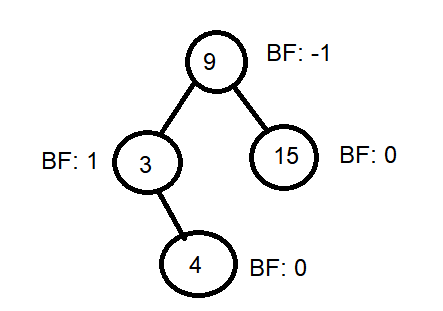
\includegraphics[width=5cm]{2C.png}
    \caption{AVL Tree with given deletion and rotation completed.}
    \label{fig:tree}
    \end{figure}

\item A single left rotation was performed, rooted at 3 (in the tree prior to the deletion).
\end{enumerate}

\end{document}